%%%%%%%%%%%%%%%%%%%%%%%%%%%%%%%%%%%%%%%%%
% baposter Portrait Poster
% Basado en el template de la clase de Aprendizaje Automático (VAE-ECG),
% adaptado al proyecto final de NLP: razonamiento latente adaptativo.
%
% baposter Class Created by:
% Brian Amberg (baposter@brian-amberg.de)
%%%%%%%%%%%%%%%%%%%%%%%%%%%%%%%%%%%%%%%%%

%----------------------------------------------------------------------------------------
%	PACKAGES AND OTHER DOCUMENT CONFIGURATIONS
%----------------------------------------------------------------------------------------

\documentclass[portrait,a0paper,fontscale=0.31]{baposter} % Adjust the font scale/size here

\usepackage[absolute,overlay]{textpos} % For absolute positioning
\usepackage{graphicx} % Required for including images
\graphicspath{{figures/}} % Directory in which figures are stored

\usepackage{amsmath} % For typesetting math
\usepackage{amssymb} % Adds new symbols to be used in math mode
\usepackage{multirow}
\usepackage{array}
\usepackage{enumitem} % Used to reduce itemize/enumerate spacing
\usepackage{booktabs} % Top and bottom rules for tables
\usepackage{palatino} % Use the Palatino font
\usepackage[font=small,labelfont=bf]{caption} % Required for specifying captions to tables and figures

\usepackage{multicol} % Required for multiple columns
\setlength{\columnsep}{1.5em} % Slightly increase the space between columns
\setlength{\columnseprule}{0mm} % No horizontal rule between columns

\usepackage{tikz} % Required for flow chart
\usetikzlibrary{shapes,arrows,positioning} % Tikz libraries required for the flow chart

\usepackage{pgfplots} % Barras de pasos por dificultad
\pgfplotsset{compat=1.18}

\usepackage{float}
\usepackage{xcolor}
\usepackage{textcomp}
\usepackage[spanish,es-noshorthands]{babel}
% Los operadores acentuados de babel-spanish (\max -> "máx") usan un helper
% frágil que rompe dentro de argumentos móviles; se desactivan globalmente.
% Ojo también: \% dentro de modo matemático rompe con babel-spanish
% ("Incompatible glue units"); escribir siempre $-32$\,\% y no $-32\,\%$.
\unaccentedoperators

\newcommand{\compresslist}{ % Define a command to reduce spacing within itemize/enumerate environments
\setlength{\itemsep}{1pt}
\setlength{\parskip}{0pt}
\setlength{\parsep}{0pt}
}

\definecolor{lightblue}{rgb}{0.145,0.6666,1} % Defines the color used for content box headers
\definecolor{udesa}{RGB}{0, 18, 187}

\begin{document}

\begin{poster}
{
headerborder=closed, % Adds a border around the header of content boxes
colspacing=1em, % Column spacing
bgColorOne=white, % Background color for the gradient on the left side of the poster
bgColorTwo=white, % Background color for the gradient on the right side of the poster
borderColor=udesa, % Border color
headerColorOne=udesa, % Background color for the header in the content boxes (left side)
headerColorTwo=udesa, % Background color for the header in the content boxes (right side)
headerFontColor=white, % Text color for the header text in the content boxes
boxColorOne=white, % Background color of the content boxes
textborder=rounded, % Format of the border around content boxes
eyecatcher=true, % Set to false for ignoring the left logo in the title and move the title left
headerheight=0.1\textheight, % Height of the header
headershape=roundedright, % Specify the rounded corner in the content box headers
headerfont=\Large\bf, % Large, bold and sans serif font in the headers of content boxes
linewidth=2pt % Width of the border lines around content boxes
}
%----------------------------------------------------------------------------------------
%	Título
%----------------------------------------------------------------------------------------
%
{
\includegraphics[height=7em]{figures/UDESA.png}} % First university/lab logo on the left
{\Large{Procesamiento del Lenguaje Natural - Universidad de San Andrés - 2026}\vspace{0.35cm}\\\huge\bf{Razonamiento latente adaptativo: \emph{halting} probabilístico tipo PonderNet sobre cadenas de pensamiento implícitas}\vspace{0.35cm}} % Poster title
{Franco Amato de Lusarreta, Valentino Arbelaiz Alberti, Naomi Couriel, Juan Cruz Giner Pulero, Ana Paula Tissera} % Author names
{} % Second university/lab logo on the right (empty)

%----------------------------------------------------------------------------------------
%	Columna 0: Introducción / Objetivos / Opción A / Referencias
%----------------------------------------------------------------------------------------

\headerbox{Introducción}{name=resumen,column=0,row=0}{

\hspace*{0.5em} Los modelos de \emph{cadena de pensamiento latente} (Coconut, CODI, SIM-CoT) razonan encadenando vectores continuos en lugar de texto, a una fracción del costo del CoT explícito. Pero fijan de antemano el número de pasos latentes $K$ y lo aplican por igual a toda entrada: un problema de dos operaciones consume el mismo presupuesto que uno de seis. Este trabajo hace ese presupuesto \textbf{adaptativo por instancia}.
}

\headerbox{Objetivos}{name=objetivos,column=0,below=resumen}{

\begin{itemize}[left=0.45em, rightmargin=0.6em]\compresslist
  \item Verificar que el presupuesto óptimo \textbf{varía por instancia} (barrido oráculo sobre CODI).
  \item Evaluar la \textbf{predicción \emph{upfront}} del presupuesto desde la consigna.
  \item Hacer adaptativo el número de pasos $K$ con \textbf{\emph{halting} probabilístico tipo PonderNet} sobre SIM-CoT/CODI (aporte central).
  \item Explorar el otro eje del presupuesto: el número de \textbf{vectores por paso} $c$.
  \item Caracterizar la \textbf{frontera exactitud--cómputo} que el $K$ fijo no puede reportar.
\end{itemize}
}

\headerbox{\textquestiondown Cuánto razonamiento?}{name=opciona,column=0,below=objetivos}{

\hspace*{0.5em} Ejecutamos CODI variando $k \in \{1,\dots,8\}$ sobre $n{=}7473$ ejemplos y medimos $k^*$: el menor $k$ que alcanza el mejor puntaje de cada instancia.

\vspace{0.3em}
\begin{center}
\small
\setlength{\tabcolsep}{3.4pt}
\begin{tabular}{lcccccccc}
\toprule
$k$ & 1 & 2 & 3 & 4 & 5 & 6 & 7 & 8 \\
\midrule
Exactitud & .41 & .43 & .48 & .58 & .64 & \textbf{.64} & .64 & .63 \\
$k^*$ (\%) & \textbf{66} & 17 & 5 & 6 & 4 & 1 & $<$1 & $<$1 \\
\bottomrule
\end{tabular}
\end{center}
\vspace{0.2em}

\hspace*{0.5em} La exactitud satura en $k{\approx}5$--$6$ ($+23$ puntos sobre $k{=}1$); el $k^*$ varía con fuerte desbalance. \textbf{Existe estructura explotable por un mecanismo adaptativo.}

\vspace{0.3em}
\hspace*{0.5em} \textbf{Resultado negativo:} un clasificador de $k^*$ sobre \emph{embeddings} congelados (MiniLM) no supera a la clase mayoritaria (el \emph{random forest} colapsa a la baseline, $0.661$; la regresión logística cae a $0.210$). La dificultad \textbf{no es legible \emph{upfront}}: la decisión debe tomarse \emph{durante} el razonamiento.
}

\headerbox{Referencias}{name=ref,column=0,below=opciona}{

\renewcommand{\section}[2]{\vskip 0.05em} % Get rid of the default "References" section title

\scriptsize
\begin{thebibliography}{9}

\bibitem{hao2024coconut}
Hao et al.
\textit{Training Large Language Models to Reason in a Continuous Latent Space} (Coconut), 2024.

\bibitem{shen2025codi}
Shen et al.
\textit{CODI: Compressing Chain-of-Thought into Continuous Space via Self-Distillation}, 2025.

\bibitem{wei2025simcot}
Wei et al.
\textit{SIM-CoT: Supervised Implicit Chain-of-Thought}, 2025.

\bibitem{banino2021pondernet}
Banino, Balaguer y Blundell.
\textit{PonderNet: Learning to Ponder}, 2021.

\end{thebibliography}
}

%----------------------------------------------------------------------------------------
%	Columna 1: Método
%----------------------------------------------------------------------------------------

\headerbox{Método: \emph{halting} adaptativo}{name=metodo,column=1}{

\hspace*{0.5em} El modelo realimenta su último estado oculto como próxima entrada ($z_k$, ``pensamientos continuos''). Una única cabeza lineal de parada decide, en cada paso, si el razonamiento acumulado ya es suficiente para responder:

\vspace{0.4em}
\begin{center}
\resizebox{\linewidth}{!}{%
\begin{tikzpicture}[>=stealth, font=\footnotesize,
  tok/.style={rectangle, rounded corners=2pt, draw=udesa, fill=udesa!8, minimum height=2.1em, inner sep=4pt},
  lat/.style={circle, draw=udesa, thick, fill=udesa!18, minimum size=2.1em, inner sep=1pt},
  hlt/.style={rectangle, rounded corners=1pt, draw=gray!70, fill=gray!12, minimum height=1.5em, inner sep=2.5pt}]
  \node[tok] (q) {pregunta $x$};
  \node[lat, right=0.55cm of q] (z1) {$z_1$};
  \node[lat, right=0.55cm of z1] (z2) {$z_2$};
  \node[right=0.4cm of z2] (dots) {$\cdots$};
  \node[lat, right=0.4cm of dots] (zk) {$z_k$};
  \node[tok, right=0.55cm of zk] (a) {respuesta};
  \draw[->, thick, udesa] (q) -- (z1);
  \draw[->, thick, udesa] (z1) -- (z2);
  \draw[->, thick, udesa] (z2) -- (dots);
  \draw[->, thick, udesa] (dots) -- (zk);
  \draw[->, thick, udesa] (zk) -- (a);
  \node[hlt, below=0.5cm of z1] (l1) {$\lambda_1$};
  \node[hlt, below=0.5cm of z2] (l2) {$\lambda_2$};
  \node[hlt, below=0.5cm of zk] (lk) {$\lambda_k$};
  \draw[->, gray!70] (z1) -- (l1);
  \draw[->, gray!70] (z2) -- (l2);
  \draw[->, gray!70] (zk) -- (lk);
  \node[below=1.35cm of dots, text=udesa] (stop) {\textbf{detener cuando} $\sum_k p_k > 0.5$};
\end{tikzpicture}
}
\end{center}
\vspace{0.2em}

\hspace*{0.5em} Cada paso emite una probabilidad de parada condicional y una respuesta candidata se decodifica tras \textbf{cada} prefijo $k=1,\dots,K$, formando la distribución de parada de PonderNet (con frontera absorbente en $K$):
\vspace{-0.2cm}
\[
  \lambda_k = \sigma\!\left(\texttt{halt\_head}(h_k)\right)
\]
\vspace{-0.75cm}
\[
  p_k = \big(\textstyle\prod_{j<k}(1-\lambda_j)\big)\,\lambda_k .
\]
\vspace{-0.5cm}

\hspace*{0.5em} El objetivo combina términos de los tres métodos: PonderNet (pérdida esperada + regularización KL), SIM-CoT (supervisión por paso) y CODI (destilación):
\vspace{-0.2cm}
\[
  \mathcal{L} = \underbrace{\textstyle\sum_k p_k\,\mathcal{L}_{\text{ans}}^{(k)}}_{\mathcal{L}_{\text{ponder}}}
  + \beta\,\mathcal{L}_{\text{step}}
  + \gamma\,\mathrm{KL}_{\text{geom}}
  + \mathcal{L}_{\text{distill}}
  + \mathcal{L}_{\text{ref}} .
\]
\vspace{-0.5cm}

\begin{itemize}[left=0.45em, rightmargin=0.6em]\compresslist
  \item El peso $\gamma$ \textbf{controla el cómputo}: regula la influencia del prior geométrico y, con ella, cuánto se acorta la cadena de razonamiento.
  \item Inferencia: se acumula la masa de parada y el bucle latente se detiene al superar un umbral (por defecto $0.5$); $K_{\max}$ actúa como límite superior.
  \item Evaluación fiel del \emph{halting}: \texttt{batch\_size}$=1$.
\end{itemize}
}

\headerbox{Prior geométrico por instancia}{name=prior,column=1,below=metodo}{

\hspace*{0.5em} Un prior global impone el mismo presupuesto esperado a todos los problemas. Lo anclamos al número de operaciones $n_i$ de cada instancia:
\vspace{-0.15cm}
\[
  \texttt{geom\_mean}_i = \mathrm{clamp}\big(\alpha\, n_i + \beta,\; \beta,\; K_{\max}\big).
\]
\vspace{-0.55cm}

\begin{figure}[H]
    \centering
    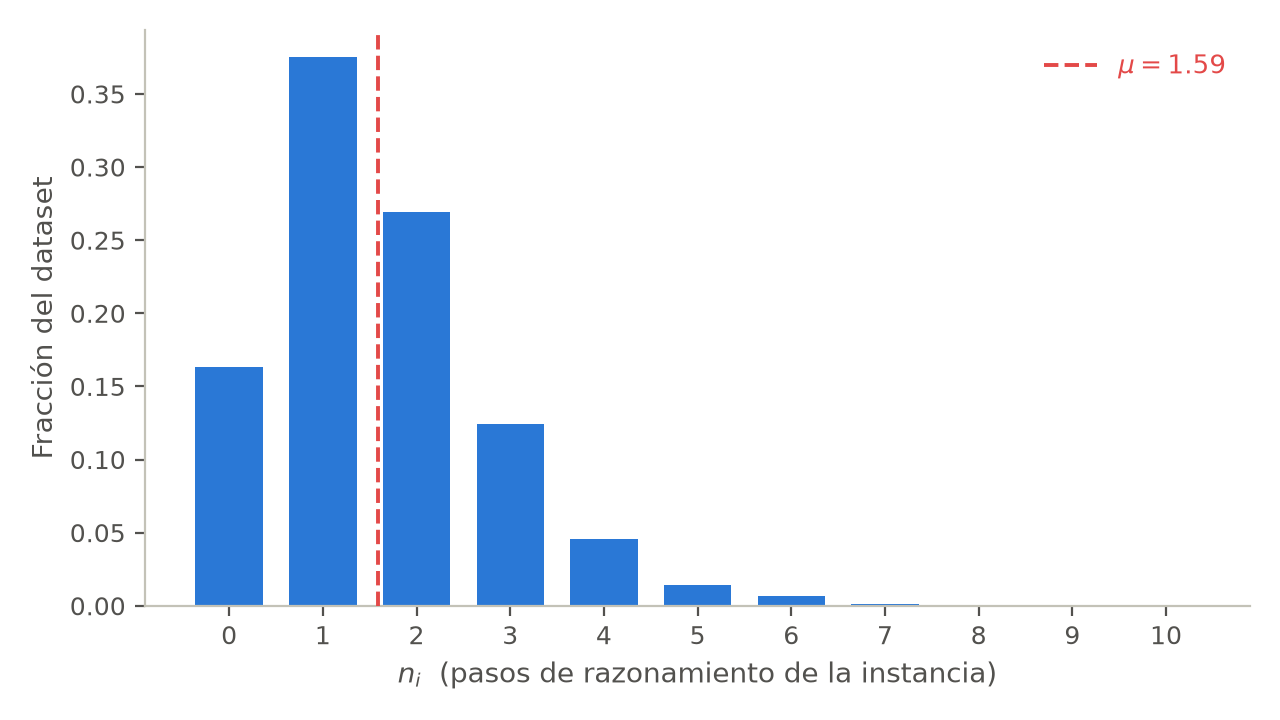
\includegraphics[width=0.64\textwidth]{ourfigures/step_distribution.png}
    \caption{Distribución de $n_i$ en GSM8k-Aug ($\mu = 1.59$): más de la mitad tiene $n_i \le 1$; el mapeo afín evita un prior degenerado.}
\end{figure}
}

%----------------------------------------------------------------------------------------
%	Columna 2: Setup / Opción B / Conclusiones / Placeholder
%----------------------------------------------------------------------------------------

\headerbox{Configuración experimental}{name=setup,column=2}{

\begin{itemize}[left=0.45em, rightmargin=0.6em]\compresslist
  \item \textbf{Datos:} GSM8k-Aug (anotaciones paso a paso de Deng et al.); subconjuntos de 15k/100k para el barrido.
  \item \textbf{Modelo:} GPT-2 (124M) + LoRA, \emph{warm-start} del checkpoint CODI de SIM-CoT (con su decoder auxiliar).
  \item \textbf{Protocolo:} exactitud \emph{greedy}, una sola pasada, \texttt{batch\_size}$=1$, sobre el \textbf{test held-out de 1319 ejemplos} (la selección de modelo se hizo en validación disjunta).
  \item \textbf{Baseline de $K$ fijo ($K{=}6$): 39.50\,\%.}
\end{itemize}
}

\headerbox{El otro eje: vectores por paso ($c$)}{name=opcionb,column=2,below=setup}{

\hspace*{0.5em} Cada paso se construye con hasta $M$ sub-vectores; un MLP destila la pérdida de reconstrucción del decoder ($\hat{\mathcal{L}} = \mathrm{MLP}(h)$) y sobrevive a inferencia: el paso termina cuando $\hat{\mathcal{L}}$ converge.

\vspace{0.3em}
\begin{center}
\small
\setlength{\tabcolsep}{4.5pt}
\begin{tabular}{lcccc}
\toprule
\textbf{Init $\times$ granularidad} & $c{=}1$ & $c{=}2$ & $c{=}3$ & $\Delta_{2\rightarrow3}$ \\
\midrule
warm $+$ atómica & 27.5 & 39.4 & 39.9 & $+0.5$ \\
warm $+$ gruesa & 25.5 & 36.6 & \textbf{40.3} & $+3.7$ \\
\emph{cold} $+$ gruesa & 5.3 & 5.5 & 5.5 & --- \\
\bottomrule
\end{tabular}
\end{center}
\vspace{0.2em}

\hspace*{0.5em} Con pasos atómicos (una operación por paso) la exactitud \textbf{satura en $c{=}2$}: la parada adaptativa no supera a la aleatoria y no hay margen explotable. Con pasos gruesos (densidad variable) la señal reaparece (adaptativo $>$ aleatorio por $2.7\sigma$), aunque modesta. \textbf{La varianza de la tarea está en el número de pasos, no en la complejidad interna de cada paso.}
}

\headerbox{Conclusiones}{name=conclu,column=2,below=opcionb}{
\vspace{0.1cm}
\begin{itemize}[left=0.45em, rightmargin=0.6em]\compresslist
    \item El \emph{halting} aprendido \textbf{iguala al baseline de $K$ fijo} ($\approx 39.5$\,\% en test) recortando \textbf{cerca de la mitad de los pasos latentes} ($3.01$ vs.\ $6$).
    \item Fuerte seguimiento de la dificultad: \textbf{Spearman $+0.675$} entre operaciones y pasos usados (test).
    \item Dos resultados negativos informativos: la dificultad no es legible \emph{upfront}; el eje $c$ no tiene margen en GSM8k-Aug.
    \item A futuro: comparación justa desde cero (en curso), otros backbones y tareas.
\end{itemize}
}

\headerbox{Ejemplo cualitativo}{name=ejemplo,column=2,below=conclu}{

\begin{center}
% PLACEHOLDER: ejemplo cualitativo del halting en acción
% (una instancia fácil que para en ~2 pasos vs una difícil que usa ~6,
% con las probabilidades de parada por paso). Generar desde una corrida
% de eval con batch_size=1 y reemplazar este recuadro.
\fbox{\parbox[c][1.9cm][c]{0.92\textwidth}{\centering
\small\textbf{[PLACEHOLDER correr]} Instancia fácil (para en $\sim$2 pasos) vs.\ difícil (usa $\sim$6), con las $\lambda_k$ por paso.
}}
\end{center}
}

%----------------------------------------------------------------------------------------
%	Resultados (banda inferior, columnas 0-2, anclada al pie)
%----------------------------------------------------------------------------------------

\headerbox{Resultados en test ($n{=}1319$): mitad del cómputo, misma exactitud}{name=resultados,column=0,span=3,above=bottom}{

\begin{minipage}[c]{0.21\textwidth}
\begin{center}
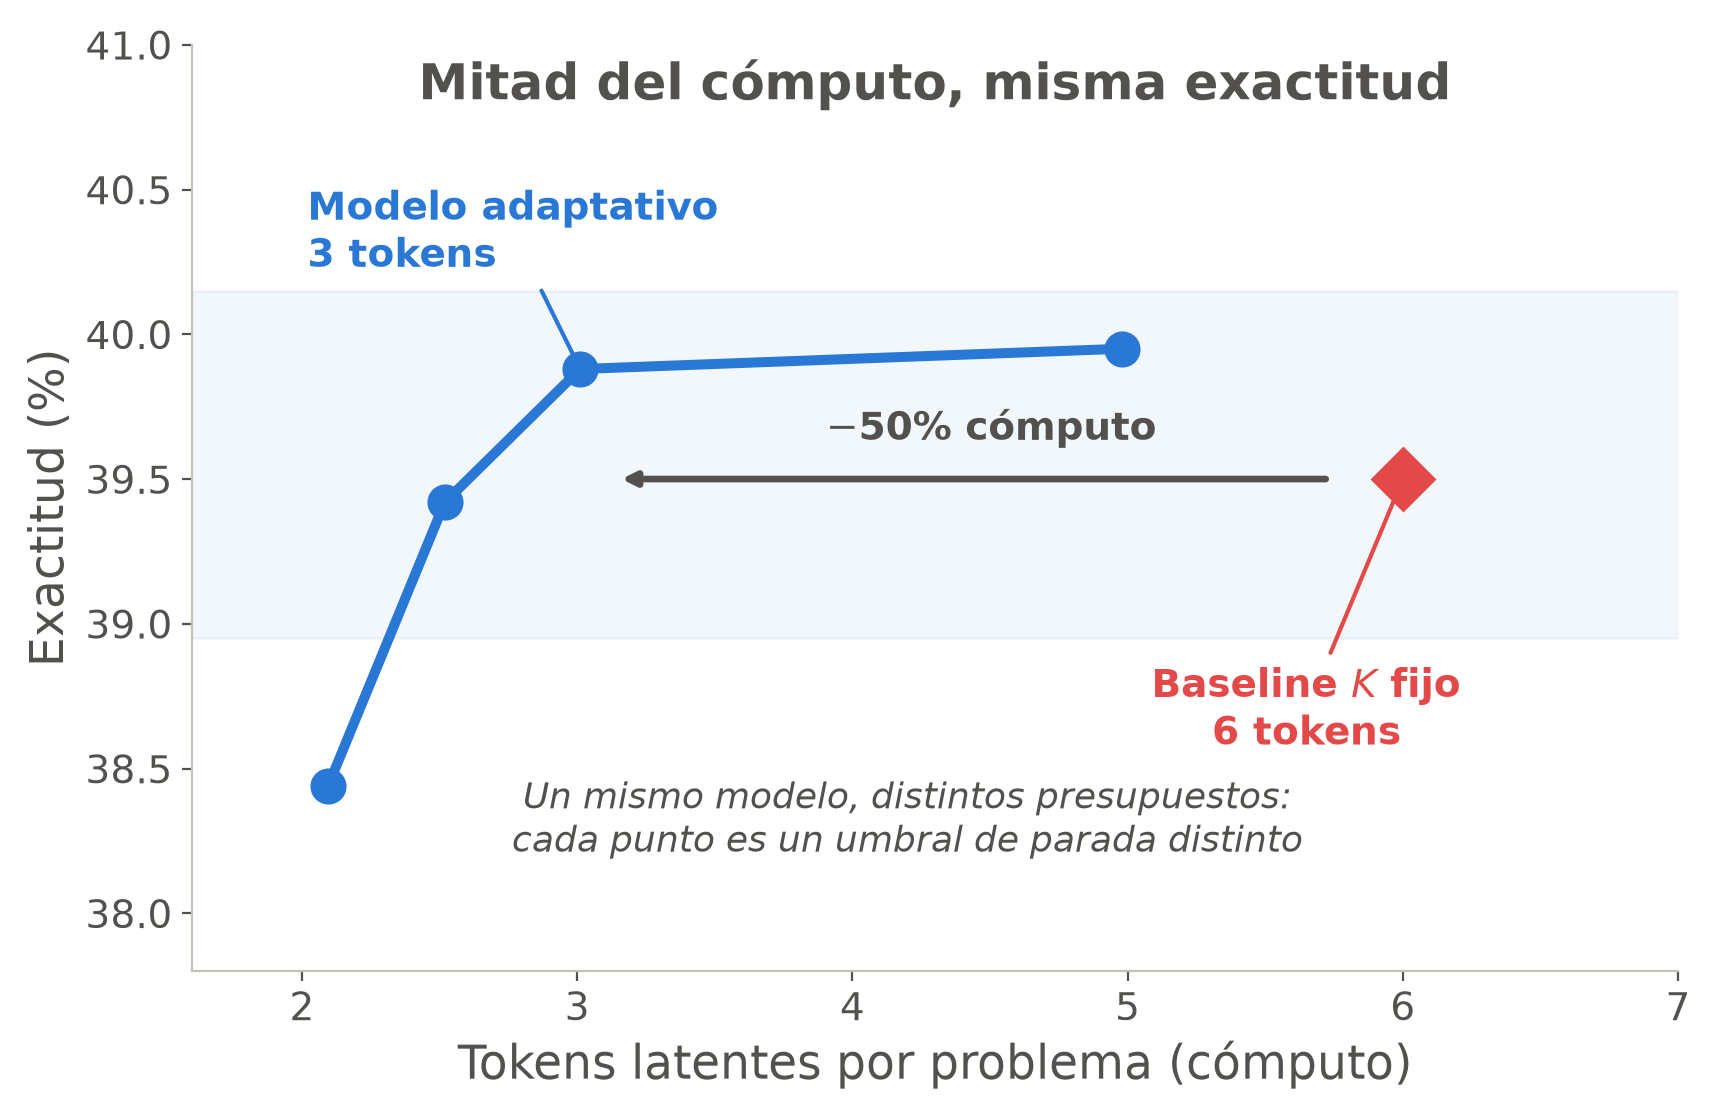
\includegraphics[width=\textwidth]{ourfigures/poster_frontier.png}

\small La frontera de M2: cada punto es el \emph{mismo} modelo con distinto umbral de parada.
\end{center}
\end{minipage}%
\hfill
\begin{minipage}[c]{0.40\textwidth}
\begin{center}
\small
\begin{tabular}{lccc}
\toprule
\textbf{Umbral} & \textbf{M0} & \textbf{M1} & \textbf{M2} \\
                & $\alpha1.0,\gamma.05$ & $\alpha1.0,\gamma.10$ & $\alpha0.6,\gamma.10$ \\
\midrule
0.3 & 39.1 @ 3.34 & 39.1 @ 2.60 & 38.4 @ \textbf{2.10} \\
0.4 & 39.6 @ 3.86 & 39.4 @ 3.16 & 39.4 @ \textbf{2.52} \\
0.5 & 40.0 @ 4.46 & 39.4 @ 3.73 & \textbf{39.9 @ 3.01} \\
0.8 & 40.2 @ 6.97 & 39.7 @ 6.39 & 40.0 @ 4.98 \\
\bottomrule
\end{tabular}

\vspace{0.4em}
\small \emph{Exactitud (\%) @ pasos latentes promedio}. M0/M1/M2 son el mismo modelo adaptativo con distinta intensidad $\gamma$ del regularizador y pendiente $\alpha$ del prior; baseline de $K$ fijo: $39.5$ @ $6.0$.
\end{center}

\vspace{0.6em}
\hspace*{0.5em} \textbf{Lectura:} la exactitud es esencialmente plana ($\sim$39--40\,\%) entre configuraciones y umbrales; la elección del punto de operación es, entonces, una decisión de \emph{presupuesto de cómputo}. El punto de mínimo cómputo a paridad es \textbf{M2 a umbral $0.5$}: $39.9$\,\% con $3.01$ pasos, la \textbf{mitad} del baseline de $K$ fijo.
\end{minipage}%
\hfill
\begin{minipage}[c]{0.28\textwidth}
\begin{center}
\begin{tikzpicture}
  \begin{axis}[
    width=\textwidth, height=5.4cm,
    ybar, bar width=8pt,
    xlabel={Operaciones ($n_{\text{expr}}$)},
    ylabel={Pasos usados},
    symbolic x coords={0,1,2,3,4,5+},
    xtick=data, ymin=0, ymax=7,
    tick label style={font=\footnotesize},
    label style={font=\footnotesize},
  ]
    \addplot[fill=udesa!60, draw=udesa] coordinates {(0,2.08)(1,2.51)(2,3.66)(3,4.76)(4,4.86)(5+,5.5)};
  \end{axis}
\end{tikzpicture}

\small Pasos promedio por dificultad (M1, umbral $0.5$, test; el grupo $5{+}$ promedia $5.2$--$5.8$). Spearman $= +0.675$: cómputo asignado por dificultad, no uniforme.
\end{center}
\end{minipage}
}

\end{poster}

\end{document}
